\chapter{Literature Review}\label{sec-literature}
\section{Space tether past missions}
This chapter is the literature survey on the following topics:
\begin{itemize}
\item Space tether past missions
\item CubeSat missions with space tether
\item Design and construction of:
\begin{enumerate}
\item Space tether deployment/retrieval system
\item Plasma contactor
\end{enumerate}
\end{itemize}

It tried to organize the past missions regarding to the space tether and the CubeSat mission in a much clear order. In the same time some historical researches about deployment/retrieval system are listed. The main point is focus on dynamics and control method of tether satellite system.
\subsection{General tether-related mission}
\begin{enumerate} 
\item{NASA}
 
NASA has been developing tether technology for space applications since the 1960s, including electrodynamic tether propulsion, the Propulsive Small Expendable Deployer System (ProSEDS) flight experiment, ” Hanging” momentum exchange tethers, rotating momentum exchange tethers and tethers supporting scientific space research. 

\item{NASA-Gemini XI} 

The Gemini XI was a manned spaceflight in NASA's Gemini program, launched on September 12,1966. One of the main objectives was related to tethers. It was synoptic terrain photography and a tethered vehicle test. The objectives were all achieved. 

\item{NASA-Gemini XII} 
   
The Gemini XII was a manned spaceflight in NASA's Gemini program launched on November 11, 1966. One of its major objectives was tethered vehicle evaluation. The objective was achieved.
\item{Tethered Payload Experiment (TPE)}

TPE-1mission was launched on January 16, 1980. Its plan was to deploy 400 metres of cable, but its deployed cable was about 38 metres. The TPE-2 mission was launched on 29 January, 1981, and its tether was deployed to a distance about 65 metres. In 1983, the TPE-3, which was also called CHARGE-1, had a length of about 500m. As the deployment system was improved, the tether deployed to its full length of 418 meters, and the tether was also found to act as a radio antenna for the electrical current through the cable. CHARGE-2 was carried out as an international program between Japan and the USA using a NASA sounding rocket at White Sands Missile Range, in December 1985, its tether deployed to a length of 426 metres.

CHARGE-2B tethered rocket mission was launched in 1992 by NASA with a Black Brant V rocket. The mission was to generate electromagnetic waves by modulating the electron beam. The tether was fully deployed over 400 meters and the experiments all worked as planned.
\item{NASA and NDRE-MAIMIK}

	The tether length of MAIMIK was about 400m. The mission was designed to study the charging of an electron-beam emitting payload using a tethered mother-daughter payload configuration. 

\item{US Air Force Geophysics Lab- Echo-7}

Designed to study the artificial electron beam propagation along magnetic field lines in space, the mission planned to study how the artificial electron beam propagates along magnetic field lines in space.
\item{OEDIPUS}

OEDIPUS-A. The conducting tether was deployed over 985 metres during the flight of a Black Brant sounding rocket in to the auroral ionosphere.

OEDIPUS-C. The following OEDIPUS mission was the OEDIPUS-C tethered payload mission, which was launched in 1995 with an 1174-metre deployed tether, and a Tether Dynamics Experiment (TDE) was also included as a part of the OEDIPUS-C.
\item{Tethered Satellite System (TSS)}

The first orbital flight experiment with a long tether was the Tethered Satellite System (TSS) mission, launched on the Space Shuttle in July 1992. The Tethered Satellite System-1 (TSS-1) was flown during STS-46, aboard the Space Shuttle Atlantis, from July 31 to August 8, 1992. The TSS-1 mission discovered a lot about the dynamics of the tethered system. Although the satellite was deployed only 260 metres, it was able to show that the tether could be deployed, controlled, and retrieved, and that the TSS was easy to control, and even more stable than predicted. The TSS was an electrodynamic tether, its deployment mechanism jammed resulting in tether sever and less than 1000 metres of deployment. The objectives of TSS-1 were 
\begin{enumerate}

\item to verify the performance of the TSS equipment; 

\item to study the electromagnetic interaction between the tether and the ambient space plasma; 

\item to investigate the dynamical forces acting on a tethered satellite. In the first tether deployment, when the satellite was moving excessively from side to side, the deployment was aborted. The second trial of deployment was unreeled to a length of 260 metres.

\end{enumerate}

In 1996, the Tethered Satellite System Reflight (TSS-1R) was carried by using US space shuttle STS-75 successfully. The primary objective of STS-75 was to carry the Tethered Satellite System Reflight (TSS-1R) into orbit and to deploy it spacewards on a conducting tether.
\item{Shuttle Electrodynamic Tether System (SETS)}

	The Shuttle Electrodynamic Tether System (SETS) experiment formed part of the scientific experiments comprising the first flight of the NASA/ASI Tethered-Satellite System flown at an altitude of 300 km and at an orbital inclination of 28.5 degrees in July/August 1992. The SETS experiment was designed to study the electrodynamic behaviour of the Orbiter-Tether-Satellite system, as well as to provide background measurements of the ionospheric environment near the Orbiter. The SETS experiment was able to operate continuously during the mission thereby providing a large data set.
\item{Small Expendable Deployer System (SEDS)}

The Small Expendable Deployer System-1 (SEDS-1) was launched from Cape Canaveral Air Force Station as a Delta/GPS secondary payload in 1993. SEDS-1 was the first successful 20-kilometre space-tether experiment. When 1 km of tether remained, active braking was applied by wrapping the tether around a "barber pole" brake. Finally, the braking system and sensors did not work as predicted, resulting in hard stop/endmass recoil at deployment completion.


The Small Expendable Deployer System-2 (SEDS-2) was launched on the last GPS Block 2 satellite in 1994. The SEDS-2 used feedback braking, which was started early in deployment. This limited the residual swing after deployment to 4 degrees. Mission success was defined as deployment of at least 18 km, plus a residual swing angle of less than 15 degrees. The SEDS-2 had an improved braking system compared to SEDS-1, which was a feedback control system and applied braking force as a function of the measured speed of the unrolling tether. This was to ensure that the satellite stopped flying out just when the whole tether was deployed and to prevent the bounces experienced during the previous mission.
\item{Plasma Motor Generator (PMG)}

In 1996, the Plasma Motor Generator (PMG) was launched by NASA. This was an electrodynamic tether, which could assess the effectiveness of using hollow cathode assemblies to deploy an ionised gas, and to "ground" electrical currents by discharging the energy to space. An early experiment used a 500 metre conducting tether. When the tether was fully deployed during this test, it generated a potential of 3,500 volts. This conducting single-line tether was severed after five hours of deployment. It was believed that the failure was caused by an electric arc generated by the conductive tether's movement through the Earth's magnetic field. The PMG flight demonstration proved the ability of the proposed Space Station plasma grounding techniques in maintaining the electrostatic potential between the Space Station and the surrounding plasma medium, the ability to use electrostatic tethers to provide thrust to offset drag in LEO space systems and the use of direct magnetic (nonrocket) propulsion for orbital maneuvering.
\item{Tether Physics and Survivability Experiment (TiPS)}

The Tether Physics and Survivability Experiment (TiPS) was deployed on June 20, 1996 at an altitude of 1,022 kilometres as a project of the US Naval Research Laboratory. The satellite was a tether physics experiment consisting of two end masses connected by a 4 km nonconducting tether. This experiment was designed to increase knowledge about gravity-gradient tether dynamics and the survivability of tethers in space.

\item{The Young Engineers's Satellite (YES)}

The first Young Engineers' Satellite (YES-1) programme was completed on November 3, 1997. It was designed to operate with a 35 km tether deployment, but the mission was cancelled before the flight when the launch authority changed the nominal Ariane orbit. In the new orbit configuration, a deployed 35 km tether would have constituted a hazard to the satellites in LEO.

The second Young Engineers Satellite (YES2) was launched on September 14, 2007. It was a technology demonstration project designed to test and produce data for the "Space Mail" concept, wherein a tether was used to return material from space to Earth, instead of by conventional chemical
propulsion. YES2 aimed to demonstrate a tether-assisted reentry concept, whereby the payload would be returned to Earth using momentum provided from a swinging tether. Deployment was intended to take place in two phases: (1) deployment of 3.5 km of tether to the local vertical and hold and (2) deployment to 30 km for a swinging cut. The measured altitude gain of the Fonton-M3 corresponded with what simulations showed would have happened if 31.7 km of tether were extended, another strong indication that the YES- 2 tether had in fact been fully depolyed.


The YES-2 mission was very nearly a complete success because of the following: (1) the entire record-breaking length of tether has been deployed; (2) Fotino rocket seemed to have been deorbited by using momentum exchange; (3) plentiful data has been gathered on tether deployment, dynamics and deorbiting, which may lead to an operational way of returning capsules without any form of propulsion

\item{The Advanced Tether Experiment (ATEx)}

The Advanced Tether Experiment (ATEx) was launched into orbit aboard the National Reconnaissance Office (NRO) sponsored by Space Technology Experiment spacecraft (STEX) on October 3, 1998. ATEx was intended to demonstrate the deployment and survivability of a novel tether design, as well as being used for controlled libration maneuvers. On January 16, 1999, after a deployment of only 22m of tether, ATEx was jettisoned from STEX due to an out-of-limit condition sent by the experiment's tether angle sensor. The ATEx lower end mass was jettisoned from the host spacecraft and the tethered upper and lower end masses freely orbited the Earth in a demonstration of long-term tether survivability. 
\item{The PICOSAT mission}

The PICOSAT mission was launched on September 30, 2001. It was a real-time tracking satellite of the miniaturized picosatellite satellite series. The name "PICO" combined the first letters of all the four of its experiments, which were the Polymer Battery Experiment (PBEX), the Ionospheric Occultation Experiment (IOX), the Coherent Electromagnetic Radio Tomography (CERTO), and the On Orbit Mission Control (OOMC). A pair of 0.25kg MEMS picosatellites with an intersatellite communications experiment were included in this mission and were connected by a 30 metre tether.
\item{Propulsive Small Expendable Deployer System (ProSEDS)--\em{Cancelled}}
	
The Propulsive Small Expendable Deployer System (ProSEDS) was a NASA space tether propulsion experiment intended to be a follow up to SEDS. It was originally intended to be flown along with a launch of a Global Positioning System (GPS) satellite in the spring of 2003, but was cancelled at the last moment, due to concerns that the tether might collide with the international space station.

\item{Multi-Application Survivable Tether (MAST)}

The Multi-Application Survivable Tether (MAST) experiment was launched into LEO on April 17, 2007, in which the 1 km multistrand interconnected tether (Hoytether) was intended to test and prove the long-term survivability of tethers in space, but the tether failed to deploy. 
\item{Tether Technologies Rocket Experiment (T-REX)}

Tether Technologies Rocket Experiment (T-REX) mission was launched August 31, 2010, on sounding rocket S-520-25, reaching a maximum altitude of 309 km. T-Rex was developed by the Kanagawa Institute of Technology/Nihon University, which led an international team to test a new type of electrodynamic tether (EDT) that may lead to a generation of propellantless propulsion systems for LEO spacecraft. The tether was 300 metres long and deployed as planned, a video of deployment was transmitted to the ground. Tether deployment was verified successfully, as was the fast ignition of a hollow cathode in the space environment.
\end{enumerate} 

\subsection{CubeSat missions with space tether}

\begin{enumerate}
\item Micro Electro-Mechanical Systems based PicoSat Inspector (MEPSI)

The MEPSI series (Micro Electro-Mechanical Systems based PicoSat Inspector) was a pair of tethered picosatellites, based on the CubeSat design, launched by a custom deployer aboard the STS-113 Endeavour mission on December 2, 2002. The two spacecrafts were cubic in shape, of mass 1 kg each, and were connected via a 15.2m tether in order to facilitate detection and tracking via ground-based radar.


\item The Space Tethered Autonomous Robotic Satellite (STARS)

On January 23, 2009, a space tether mission called "The Space Tethered Autonomous Robotic Satellite (STARS)," developed by Kagawa Satellite Development Project at Kagawa University, was launched as a secondary payload aboard H-IIA flight. The satellite was named KUKAI after launch and based on a "cubesat" platform like MAST, and consisted of two subsatellites, "Ku" and "Kai," which are linked by a 5-meter tether. The separation of the rocket and satellite and the transfer into the planned orbit were successful, but the tether—only deployed to a length of several centimeters because of the launch lock trouble of the tether reel mechanism .

\item Tether Electrodynamic Propulsion CubeSat Experiment (TEPCE)

Tether Electrodynamic Propulsion CubeSat Experiment (TEPCE) mission, planned by Naval Research Laboratory, is an electrodynamic tether experiment based on a "triple cubesat" configuration. This experiment is currently planned for launch as a secondary payload in September 2013. Two nearly identical endmasses with a stacer spring between them are used in TEPCE, which separate the endmass and start deployment of a 1 km long braided-tape conducting tether. TEPCE will use a passive braking to reduce speed and hence recoil at the end of electrodynamic current in either direction.
The main purpose of this mission is to raise or lower the orbit by several kilometres per day, to change libration state, to change orbit plane, and to actively maneuver.
\end{enumerate}
\begin{figure}[ht]
\centering
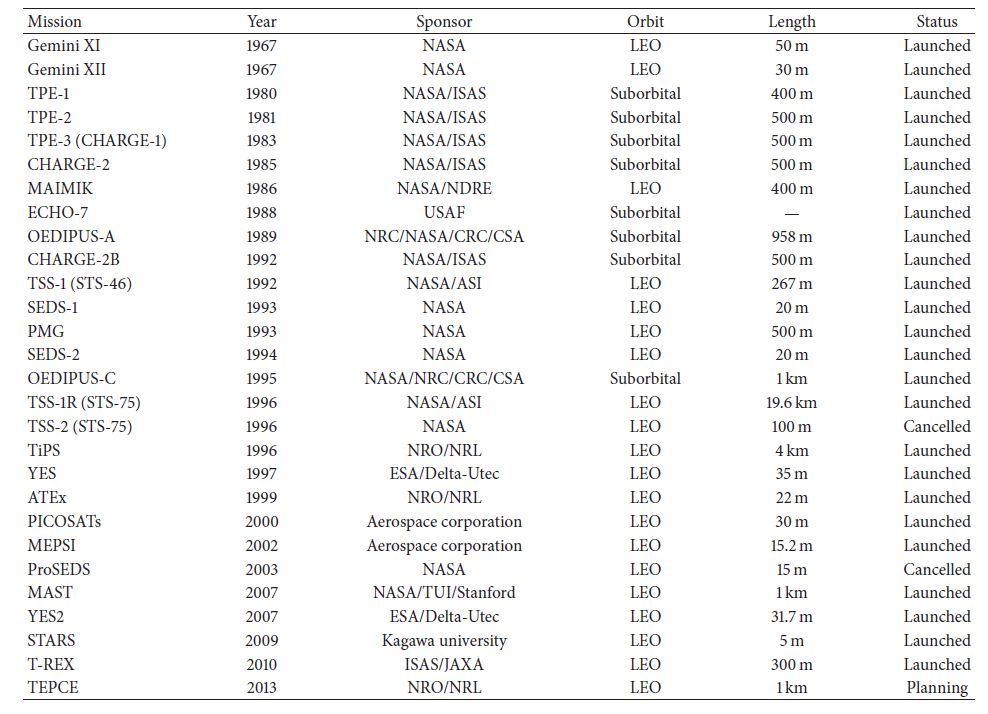
\includegraphics[width=\textwidth]{fig/LiteratureReview/TetherMissionHistory}
\caption{Tether mission history}
\label{Lit-TetherMissionHistory}
\end{figure}


\section{Design and construction}

\subsection{Space tether deployment/retrieval system}
Besides other operational phases, a TSS mission launch always involves both deployment and retrieval. Tether retrieval is the opposite of deployment and is equally important in dynamical terms. Tether deployment and retrieval are two of the most important steps in space tether applications. The following contents introduce some interesting things about the deployment and retrieval.

\begin{figure}[ht]
\centering
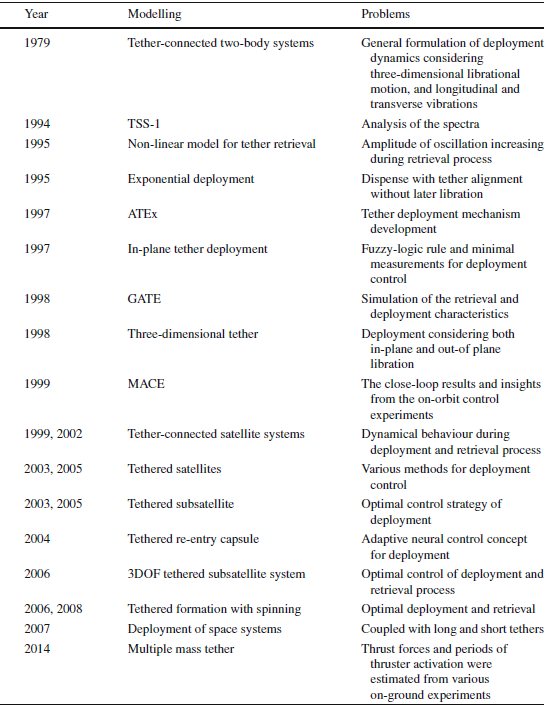
\includegraphics{fig/LiteratureReview/DeploymentAndRetrieval}
\caption{Summary of tether deployment and retrieval}
\label{Lit-DeploymentAndRetrieval}
\end{figure}

\begin{enumerate}

\item ATEx design iterations \\
In 1997, Koss described the tether deployment mechanism development for the Advanced Tether Experiment (ATEx) mission with some design iterations, which included: energetic(spring) deployment, a DC brush motor-driven deployment mechanism and a stepper motor-driven deployment mechanism

\item Fuzzy-logic feedback deployment control\\
A tethered system deployment control by fuzzy-logic feedback was proposed by Licata in 1997, in which the feedback control was based on a simple fuzzy-logic rule and minimal measurements for in-plane tether deployment control problems. The fuzzy-logic law, for the proposed rate feedback control solution to the in-plane deployed tether terminal position-only problem has been associated with the tether length-angle state plane, or the physical deployment trajectory plane.

\item Using Active Reel Type Deplorer to retrieve and deploy tether\\
Carter and Greene studied the simulation of the retrieval and deployment characteristics for the Getaway Tether Experiment (GATE) in 1998. The GATE was a single tether satellite system for the study of tether dynamics and electrodynamic technology. One goal of GATE was to measure and control tether disturbances by micro meteorite impact using an active reel type deplorer, which was able to retrieve and deploy the tether. A closed-loop controller for the tethered system was given, which allowed the tether to be actively reeled in (retrieval) or passively reeled out (deployment), to and from the mother subsatellite.

\item Strategies for TSS retrieval-tension control in the tether\\
The dynamical behaviour of tether-connected satellite systems during the deployment and retrieval process was studied by Djebli et al. in 1999 and 2002.The system consisted of a space station connected to a subsatellite by means of a tether of variable length. A simplified model was given in which the space station and the subsatellite were reduced to material points and the system mass centre moved along a circular orbit with three-dimensional transverse and longitudinal oscillations. Strategies for retrieval were obtained in order to increase the tension in the tether at the final stage of retrieval. These laws of retrieval were deduced from the laws obtained in a previous paper for the particular case of a massless tether. Retrieval of a subsatellite to a larger vehicle was examined by Djebli et al. in 2002, which concentrated on laws for retrieval and deployment, combining 'simple' linear and 'fast' laws. This would be applicable to passive momentum exchange tethers and potentially to ED tethers.


In 2006 and 2008, Williams published his works on the optimal deployment and retrieval for a tethered formation with spinning in the orbital plane, in which a tethered formation was modelled by point mass satellites and connected via inelastic tethers. The optimal deployment and retrieval trajectories using tension control were developed for different spinning conditions.


\item Viscoelastic space billiard model\\
In 2003 and 2005, Barkow et al. published three papers on various methods used for controlling the deployment of tethered satellites. The deployment of a tethered satellite system is one of the most critical
phases in a tether mission. Based on a viscoelastic space billiard model, a targeting strategy
was developed which made use of the system's chaotic nature and allowed the system to be steered into its equilibrium faster and more efficiently, when compared to conventional strategies.

\item Optimal control\\
In 2003, Steindl and Troger proposed their works that the optimal control of deployment of a tethered subsatellite moving on a circular orbit around the Earth, in which an optimal control of deployment andretrieval of a tethered subsatellite from a main satellite was treated.
Jin et al. presented an optimal control of the deployment and retrieval processes of a three degree
of freedom (DOF) tethered subsatellite system using truncated Chebyshev series to approximate the state
variables.

\item Adaptive neural control\\
An adaptive neural control concept for the deployment of a tethered re-entry capsule was developed by
Glabel et al. in 2004, in which the indirect neural controller combined two neural networks, a controller network and a plant model network. After introducing the tether deployment scenario, assumptions and simplifications were applied to the mathematical system model. The simulation results allowed a performance comparison of the linear quadratic regulator and the neural control concept.
\item Tether length factor\\
In 2007, Mantri's research aimed to model and understand the deployment of space systems with long
and short tethers, which was divided into two parts. The models are set for different length tether systems 

\item Spool-type reel using thruster \\
In 2014, Iki et al. investigated an ED tether deployment from a spool-type reel using thrusters with
a length of several kilomerters, in which the deployment of multiple mass tether deployment was studied
the key parameters of a multiple mass tether model. The key parameters of the thrust forces and periods
of thruster activation were estimated from various on-ground experiments.

\end{enumerate}



\subsection{Space tether dynamical modelling}

Different models are used for different purposes. In order to solve different problems, several dynamical models have been proposed. Here are the recent proposed models, from 2001 to 2014.\\
According to the problem, different level models are proposed. From simple to complex, Non-dissipative massive Tether, electrodynamic tether, tether satellite system(TSS), advanced safety tether Operation and Reliability(ASTOR)and motorized momentum exchange tether(MMET) are the objects. And according to the problem, you can you the model like slack-sprint model, dumbbell model, flexible model, ponderable tether model, two mass point with the rigid rod model and so on. 


\begin{figure}[ht]
\end{figure}

\begin{table}[h!]
\renewcommand\arraystretch{2}
	
	\begin{center}
	
	\caption{Physical Modeling Method for different problems}
	\begin{tabular}{p{0.2\linewidth}|p{0.1\linewidth}|p{0.25\linewidth}|p{0.45\linewidth}}
	\toprule
	\textbf{Author} & \textbf{Year} & \textbf{Modelling Method} & \textbf{What problem to solve}\\
	\midrule
	Cartmell, Ziegler & 2001 & Scale model of MMET & \\
	Chen and Cartmell, Chen and Ismail & 2001-2012 & MMET series models & Dynamical modelling and control\\
	Mazzoleni and Hoffman & 2001 & Tethered artificial gravity satellite & Non-planar spin-up dynamics\\
	Ellis and Hall&	2010&	Two Point masses connected by rigid rod & Out-of-plane librations\\
	Aslanov &	2010&	Rigid body TSS system	& Plane translational motion and rotational motion\\
	Zanutto et al.& 2011 & Electrodynamic tether & Perturbed classical three-body problem\\
	Kristiansen et al.&	2012 &	Non-dissipative massive tether & Orbital motions\\
	Zhao et al.	&2012&	Dumb-bell TSS & Analytical first-order solutions of the librational angles\\
	Jung et al. & 2014 &	TSS with a moving mass & Libration angle with respect to the system parameters\\
	\bottomrule

	\end{tabular}
	
	\end{center}
\end{table}



\newpage
